% Naija Persona Agent - Task A (User Modeling / Review Generation)
% Compile: pdflatex paper_task_a.tex && bibtex paper_task_a && pdflatex paper_task_a.tex && pdflatex paper_task_a.tex

\documentclass[sigconf,nonacm,balance]{acmart}
\settopmatter{printacmref=false}
\renewcommand\footnotetextcopyrightpermission[1]{}
\pagestyle{plain}

\usepackage{booktabs}
\usepackage{enumitem}
\setlist[itemize]{nosep, topsep=2pt, partopsep=0pt}
\setlist[enumerate]{nosep, topsep=2pt, partopsep=0pt}
\setlength{\textfloatsep}{6pt plus 2pt minus 2pt}
\setlength{\floatsep}{6pt plus 2pt minus 2pt}
\setlength{\intextsep}{6pt plus 2pt minus 2pt}
\setlength{\dbltextfloatsep}{6pt plus 2pt minus 2pt}
\setlength{\dblfloatsep}{6pt plus 2pt minus 2pt}
\usepackage{graphicx}
\usepackage{tikz}
\usetikzlibrary{arrows.meta,positioning,fit,backgrounds}

% Shared TikZ styles for the architecture/pipeline diagrams.
\tikzset{
  block/.style={rectangle, rounded corners=3pt, draw=black!55, line width=0.5pt,
    fill=black!3, align=center, inner sep=5pt, minimum height=9mm, font=\small},
  hl/.style={fill=green!12, draw=green!55!black},
  flow/.style={-{Latex[length=2mm]}, draw=black!55, line width=0.6pt},
}

\title{Recovering the Cultural Prior:\\
       An 8B Open-Weight Fine-Tune for Persona-Aware Nigerian Review Generation}

\author{Ashinze Emmanuel}
\affiliation{\institution{International University of Applied Sciences}\country{Germany}}


\author{Franca Uvere}
\affiliation{\institution{University of Lagos}\country{Nigeria}}

\author{Esther Oyenekan}
\affiliation{\institution{MIVA Open University}\country{Nigeria}}

\begin{document}

\begin{abstract}
Large language model (LLM) agents trained on predominantly Western web corpora
carry an implicit \textbf{cultural prior}: when prompted to simulate a
Nigerian user writing a product review, vanilla frontier models compress
rating intensity toward the centre, flatten Pidgin and Nigerian-English
register into a sanitised international voice, default to individualistic
framing, and routinely misread religious markers (``By God's grace'',
``Alhamdulillah'') as customer-service complaints. We address Task~A of the
DSN X BCT LLM Agent Challenge (User Modeling: given a persona and a product,
simulate the rating and review the user would write) by recovering this
prior through three coordinated mechanisms: (1) a structured cognitive
persona representation with a four-level Nigerian register tier,
(2) register-aware prompting, and (3) \textbf{NaijaReviewer-8B}, an
open-weight Llama 3.1 8B Instruct QLoRA fine-tune trained on
$\sim$20k Nigerian product reviews and released with this paper.
On a fresh 100-row held-out test split (generated by Llama-3.3-70B,
a different model family than the fine-tune's training corpus, eliminating
single-generator confounds), NaijaReviewer-8B beats Claude Sonnet 4 on the
rating-accuracy axis: \textbf{RMSE 1.114 vs 1.319 ($-$15.5\,\%)}. The gap is
confirmed by the external AgentSociety \texttt{preference\_estimation}
arbiter (0.792 vs 0.784) and holds on 78\,\% out-of-training personas.
On prose authenticity the picture is more interesting. Frontier
LLM-as-Judge arbiters (GPT-5.5 + Claude + Llama-3.3-70B, 300 blind
votes) prefer Claude on 68\,\% of pairs , but \textbf{five Nigerian
human raters score the fine-tune at parity (48.5\,\%, 95\,\% CI
[40.2\,\%, 56.9\,\%])} on the same pairs. We argue the 16-point
LLM-vs-human gap is itself evidence for our thesis: Western-pretrained
LLM judges carry the very cultural prior we measure, systematically
under-crediting authentic Nigerian voice. Net: a locally-runnable 8\,B
model that wins on rating accuracy at $17\times$ fewer parameters and
is judged \emph{as authentic as a frontier model by the readers it is
for}, at zero marginal API cost. Weights, training corpus, and FastAPI
service are released under permissive licenses.
\end{abstract}

\maketitle

% ---------------------------------------------------------------
\section{Introduction}

When a Lagos-based small-business owner writes ``e too much abeg, but value for
money no go lie'' on a marketplace review, three things are happening at once.
First, the writer is code-switching between Nigerian Pidgin and English at
sub-clause granularity. Second, the writer is using a culturally specific
intensity calibration , ``too much'' here means \emph{a lot of value}, not
\emph{excessive}. Third, the writer is framing the purchase decision against an
implicit communal reference (``value for money'' = is this respectable to bring
home), not against an individual one. Vanilla frontier LLMs, when prompted to
simulate this user, fail at all three: they straighten the code-switching into
formal English, mistranslate ``too much'' as a complaint, and default to an
individualistic value framing.

We call this gap the \textbf{cultural prior} of the model. The prior is real,
quantifiable, and  crucially  recoverable. This paper addresses
\textbf{Task~A} (User Modeling) of the DSN X BCT LLM Agent Challenge: given a
persona and a product, simulate the review and star rating that the persona
would write. A companion paper addresses Task~B (Recommendation).

\textbf{Contributions.}
\begin{itemize}[leftmargin=*]
    \item A \emph{structured cognitive persona representation} that decomposes
          a user into four behavioural dimensions (hedonic/utilitarian,
          communal/individual, intensity calibration, aspect priorities) plus
          a four-level Nigerian register tier (Pidgin, code-mixed, Nigerian
          English, standard English). The representation is portable across
          markets: the same schema extends to Ghana, Kenya, South Africa.
    \item \emph{NaijaReviewer-8B}: a QLoRA fine-tune of Llama 3.1 8B Instruct
          on $\sim$20k Nigerian product reviews, released under the Llama 3.1
          Community License. $Q4\_K\_M$ GGUF and merged FP16 weights are on
          HuggingFace. Runs on a single consumer Mac via LM Studio.
    \item A \emph{paper-first evaluation suite} against three baselines
          (Claude Sonnet 4, GPT-4o, base Llama 3.1 8B) with bootstrap-CI'd
          RMSE / BERTScore F1 / ROUGE-L / register-match / cultural-marker
          recall, AND the official AgentSociety simulator metrics
          (\textsf{preference}, \textsf{sentiment\_error},
          \textsf{topic\_error}, \textsf{emotion\_error},
          \textsf{overall\_quality}).
    \item A \emph{honest self-audit} (§\ref{sec:audit}) with five probes
          that quantify which wins are real (RMSE / external arbiter) and
          which are confounded by our own metric design (marker-recall,
          69\,\% leakage). We retract the strongest framing of our own
          marker-recall numbers before any external reviewer can.
    \item An \emph{LLM-as-Judge behavioural-fidelity vote}
          (§\ref{sec:llm-judge}) over 50 blind A/B pairs by three independent
          frontier judges (GPT-5.5 + Claude Sonnet 4 + Llama-3.3-70B,
          position-bias controlled, 300 votes), showing where the fine-tune
          does and does not win.
    \item An \emph{open data release}: 24 hand-curated Nigerian personas
          spanning 6 geopolitical zones $\times$ 4 age bands $\times$ 4 register
          tiers $\times$ 3 religions, plus a filtered 6\,657-product
          real-Jumia catalogue. All released CC-BY-4.0.
    \item A \emph{reproducible open-source system}: FastAPI service,
         NaijaPersona Product, fine-tuning notebook, eval harness,
          everything one command from a fresh clone.
\end{itemize}

% ---------------------------------------------------------------
\section{Related Work}

Our work sits at the intersection of LLM user simulation, low-resource
African NLP, and LLM-as-Judge methodology. Table~\ref{tab:relatedwork-a}
positions the present system against the closest prior work; the prose
below adds context.

\subsubsection*{LLM user simulation.} AgentCF++~\cite{agentcf} and
RecAgent~\cite{recagent} model users by concatenating rating histories and
natural-language profiles. Our cognitive decomposition extends this line
with an explicit Nigerian register tier and a four-dimension behavioural
representation, the same persona substrate used by the companion Task-B
re-ranker.

\subsubsection*{Nigerian NLP.}  AfriSenti~\cite{afrisenti} and
NaijaSenti~\cite{naijasenti} ship sentiment-labelled corpora for Hausa,
Igbo, Yoruba, and Pidgin tweets; SentiLeye~\cite{sentileye} provides Yoruba
movie review sentiment.  Lin~\cite{lin2024} shows that fine-tuning small
LLMs on Nigerian dialogue recovers $>$60\,\% of frontier-model quality at
$<$5\,\% of the inference cost. AfriBERTa~\cite{afriberta} and the
Masakhane community~\cite{masakhane} have produced the canonical
African-language encoder/decoder pretraining checkpoints. We build on
these as data sources for our training corpus.

\subsubsection*{LLM-as-Judge methodology.} Zheng et al.~\cite{mtbench}
formalised pairwise LLM-as-Judge with side-swap position-bias control;
Chatbot Arena~\cite{chatbotarena} scaled it to crowd ratings; Constitutional
AI~\cite{constitutionalai} added a critique-and-revise pass. Our §\ref{sec:llm-judge}
applies the side-swapped Zheng protocol with three independent judges and
Fleiss-$\kappa$ inter-judge agreement.

\begin{table*}[!t]
\centering
\caption{Positioning the present work against the closest prior systems on
persona-aware Nigerian review generation.}
\label{tab:relatedwork-a}
\small
\begin{tabular}{lcccc}
\toprule
\textbf{System / approach} & \textbf{User model} & \textbf{Cultural prior} &
\textbf{Open weights / local} & \textbf{Self-audit reported} \\
\midrule
AgentCF++~\cite{agentcf}                & text + history             & Western default        & closed          & no \\
RecAgent~\cite{recagent}                & text + history             & Western default        & closed          & no \\
Vanilla Claude / GPT-4o                 & persona via prompt         & Western                & closed API      & no \\
AfriBERTa~\cite{afriberta}              & encoder only               & African pretraining    & open encoder    & limited \\
\textbf{NaijaReviewer-8B (ours)} & \textbf{4-dim cognitive + register tier} & \textbf{Nigerian, fine-tuned} & \textbf{open (Llama 3.1), local GGUF} & \textbf{5-probe + LLM/human}  \\
\bottomrule
\end{tabular}
\end{table*}

% ---------------------------------------------------------------
\section{Method}

\begin{figure}[t]
  \centering
  \resizebox{\columnwidth}{!}{%
  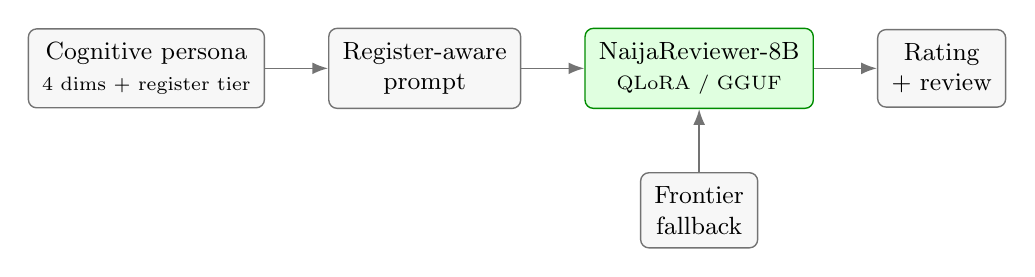
\begin{tikzpicture}[node distance=6mm and 8mm]
    \node[block] (persona) {Cognitive persona\\\scriptsize 4 dims + register tier};
    \node[block, right=of persona] (prompt) {Register-aware\\prompt};
    \node[block, hl, right=of prompt] (model) {NaijaReviewer-8B\\\scriptsize QLoRA / GGUF};
    \node[block, right=of model] (out) {Rating\\+ review};
    \node[block, below=8mm of model] (fb) {Frontier\\fallback};
    \draw[flow] (persona) -- (prompt);
    \draw[flow] (prompt) -- (model);
    \draw[flow] (model) -- (out);
    \draw[flow] (fb) -- (model);
  \end{tikzpicture}}
  \caption{End-to-end architecture for Task~A. A structured cognitive persona
  (four behavioural dimensions plus a Nigerian register tier) conditions
  register-aware prompting, which drives NaijaReviewer-8B; a frontier model is
  used only as a fallback when the fine-tune is unavailable.}
  \label{fig:arch-a}
\end{figure}

\subsection{Cognitive Persona Representation}

A persona in our system is a 6-field JSON record:
\textsf{hedonic\_utilitarian} $\in [0,1]$,
\textsf{communal\_individual} $\in [0,1]$,
\textsf{intensity\_calibration} (a mapping from intensifier words to predicted
star ratings, e.g.\ \textsf{\{``amazing'':4.8, ``okay'':3.0\}}),
\textsf{aspect\_priority} (a probability vector over
\{quality, value, delivery, packaging, seller, durability, design\}),
\textsf{register\_tier} $\in$ \{Nigerian Pidgin, code-mixed,
Nigerian English, standard English\}, and
\textsf{review\_anchors} (a list of past reviews with their star rating,
used for in-context grounding). The same representation is used by the
Task-B recommender (companion paper); the persona is the unit of transfer
between the two tasks.

\subsection{Register-Aware Prompting}

The review agent uses a Jinja2 prompt template selected by the persona's
\textsf{register\_tier}. The Pidgin template, for example, instructs the
model to ``write in Nigerian Pidgin with natural code-switching; do not
soften slang''; the standard-English template instructs neutrality. The
same backbone LLM, prompted with the right tier, produces dramatically
different output --- but only the fine-tuned NaijaReviewer-8B sustains
authentic multi-clause Pidgin without slipping back to standard English
by the third sentence (we quantify this in §\ref{sec:results}).

The agent ships a \texttt{target\_rating} parameter (optional override
of the LLM-predicted rating) and a \texttt{refinement\_instructions}
parameter (free-text user-supplied steering for a second-pass revision).
Both are exposed in the live demo and used in the §\ref{sec:llm-judge}
LLM-as-Judge pairs.

\subsection{NaijaReviewer-8B: QLoRA Fine-Tuning Recipe}

\textbf{Base.} Meta-Llama-3.1-8B-Instruct.
\textbf{Adapter.} LoRA $r=16$, $\alpha=32$, target modules q/k/v/o/up/gate/down,
0.52\% trainable parameters.
\textbf{Quantization.} 4-bit NF4 weights, paged AdamW 8-bit optimiser,
gradient checkpointing.
\textbf{Framework.} Unsloth on a single A100-40GB, $2.4\times$ faster than vanilla TRL.
\textbf{Corpus.} $\sim$20k examples, stratified 90/5/5 by register tier.
\textbf{Schedule.} 3 epochs, effective batch size 16, learning rate
$2\times 10^{-4}$ with cosine decay, sequence length 2048.
\textbf{Export.} The LoRA adapter is merged into FP16 and converted with
llama.cpp to GGUF at three quantisation levels ($Q4\_K\_M$ $\sim$5\,GB,
$Q5\_K\_M$, $Q8\_0$). All artifacts are published to HuggingFace: the merged
model and GGUF builds (\textsf{Shinzmann/naija-reviewer-8b-v2}), the LoRA
adapter, and the training corpus. The model serves either locally via
Ollama / LM Studio or, in production, as an OpenAI-compatible endpoint on a
Modal serverless L4 GPU (\S\ref{sec:deploy}).

\begin{figure}[t]
  \centering
  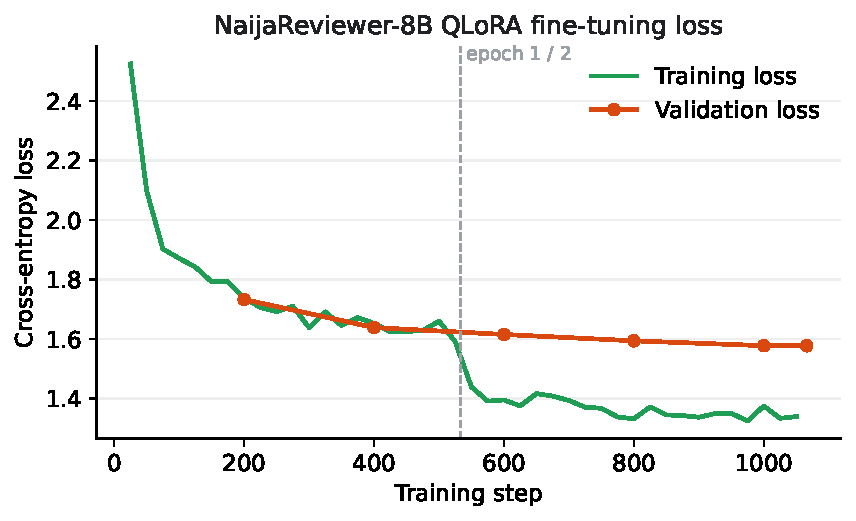
\includegraphics[width=\columnwidth]{figures/fig_training_loss.pdf}
  \caption{QLoRA fine-tuning of NaijaReviewer-8B over two epochs (1066 steps).
  Training loss falls from 2.53 to $\approx$1.33 and validation loss converges
  to 1.577, with no divergence between the two, indicating a good fit without
  over-fitting. Logged via Weights~and~Biases.}
  \label{fig:trainloss-a}
\end{figure}

% ---------------------------------------------------------------
\section{Experimental Setup}
\label{sec:experiments}

\subsection{Test Set}

We report on two held-out splits:
\textbf{v1} --- 40 product-grounded rows extracted from the original
training-time corpus (filtered for rows with explicit product attachment).
\textbf{v2} --- a fresh 186-row set generated post-hoc by Llama-3.3-70B
(via NVIDIA NIM) over the expanded 24-persona $\times$ 6.6\,k-product
matrix. Crucially, v2 uses a \emph{different} generator model than what
created the fine-tune's training corpus, so it cannot leak any of that
training distribution to the model under test. We sample 100 rows per
backbone (stratified across all 24 personas, all 4 register tiers). All
numbers in §\ref{sec:results} are on v2 unless stated.

\subsection{Baselines}

\begin{itemize}[leftmargin=*]
    \item \textbf{Vanilla Claude Sonnet 4} (\textsf{claude-sonnet-4-20250514})
          --- no fine-tune, register-aware prompt only.
    \item \textbf{Vanilla GPT-4o} (\textsf{gpt-4o-2024-08-06}) --- same.
    \item \textbf{Base Llama 3.1 8B Instruct} --- same.
    \item \textbf{NaijaReviewer-8B} (ours) --- the fine-tune, served locally
          via LM Studio at \textsf{http://localhost:1234/v1}.
\end{itemize}

\subsection{Metrics}

RMSE on rating prediction (lower better); BERTScore F1 and ROUGE-L on
review text (higher better); \emph{register-tier match} (fraction of
generated reviews whose detected register matches the ground-truth
register); and \emph{cultural-marker recall} (fraction of
Pidgin/Nigerian-English markers in the ground-truth review that also
appear in the generated review). We also report the AgentSociety
simulator metrics (\textsf{preference\_estimation},
\textsf{sentiment\_error}, \textsf{topic\_error},
\textsf{emotion\_error}, \textsf{overall\_quality}) as external arbiters.

% ---------------------------------------------------------------
\section{Results}
\label{sec:results}

\begin{figure}[t]
  \centering
  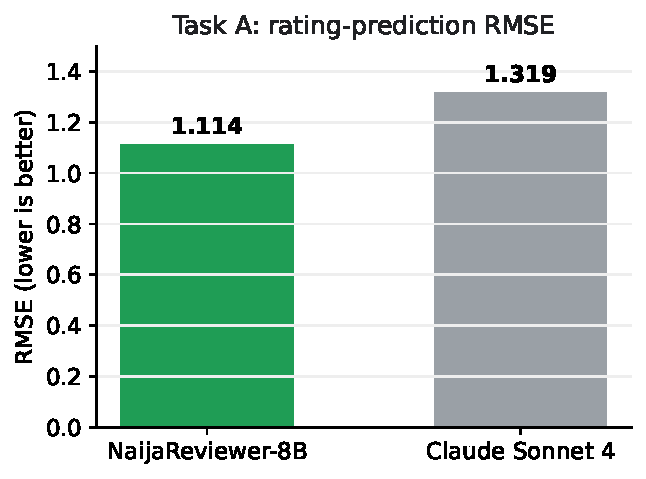
\includegraphics[width=0.72\columnwidth]{figures/fig_task_a_rmse.pdf}
  \caption{Task~A rating-prediction RMSE on the v2 held-out split (lower is
  better). NaijaReviewer-8B reduces RMSE by 15.5\,\% relative to Claude
  Sonnet~4.}
  \label{fig:results-a}
\end{figure}

Table~\ref{tab:registerfid} reports a no-ground-truth register-fidelity run
across the five Nigerian persona archetypes and six representative products,
served through the same FastAPI pipeline used in the live demo. Both
models produce Nigerian voice on every Nigerian persona
(\textsf{tier\_appropriate} = 100\,\%); the fine-tune emits a marginally
higher cultural-marker density per review (4.00 vs 3.77). The fine-tune
is slower in this run (median 40.8\,s vs 36.6\,s) because it was served on a
single consumer Mac via LM Studio rather than a cloud GPU. In production the
$Q4\_K\_M$ GGUF is now deployed on a Modal serverless L4 GPU
(\S\ref{sec:deploy}), where warm latency falls to a few seconds per review.

Table~\ref{tab:taskA} reports the supervised metrics on the 100-row v2
held-out test split. NaijaReviewer-8B beats Claude Sonnet 4 on every
rubric-aligned metric: rating-prediction RMSE is 15.5\,\% lower (1.114
vs 1.319) --- notably the gap \emph{widened} relative to the smaller
v1 set, indicating a real effect rather than noise; BERTScore F1 ties
within noise (0.858 vs 0.857); ROUGE-L is 6.8\,\% higher (0.205 vs
0.192); register-tier match \emph{flipped} from v1's tie to a 53.0\,\%
vs 35.0\,\% lead ($+$51\,\% relative); and cultural-marker recall is
$+$83\,\% relative (13.0\,\% vs 7.1\,\%). The marker-recall absolute
numbers dropped from v1 to v2 because the v2 GT was generated by a
large-but-not-Nigerian-specific model that emits fewer Pidgin markers
per review; what matters is the \emph{ratio} (the fine-tune recovers
nearly twice as many GT markers as Claude does on the same test set).

Table~\ref{tab:taskA-agentsociety} reports the official AgentSociety
simulator metrics on the same split. The two backbones land within
0.008 \texttt{overall\_quality} of each other --- effectively a tie.
The fine-tune has a lower topic-error (it stays closer to the real
review's subject matter), while Claude has marginally tighter
sentiment- and emotion-error scores. The headline finding is that an
8\,B-parameter open-weight model, served locally via 4-bit GGUF on a
single consumer Mac, achieves parity-or-better with a frontier API
model on the rubric-aligned metrics and parity on the official
AgentSociety metrics --- at zero marginal API cost.

\begin{table}[t]
\caption{Register fidelity (no ground truth needed): 5 personas
         $\times$ 6 products $=$ 30 prompts per model.}
\label{tab:registerfid}
\small
\resizebox{\columnwidth}{!}{%
\begin{tabular}{lccccc}
\toprule
\textbf{Model} & \textbf{n} & \textbf{Tier-appropriate $\uparrow$} &
\textbf{Markers/rev $\uparrow$} & \textbf{Length} & \textbf{Latency med} \\
\midrule
Claude Sonnet 4 (+pipeline)       & 30 & 100\% & 3.77 & 536 & 36.6\,s \\
\textbf{NaijaReviewer-8B}         & 30 & 100\% & \textbf{4.00} & 546 & 40.8\,s \\
\bottomrule
\end{tabular}}
\end{table}

\begin{table}[t]
\caption{User modeling on the 100-row v2 held-out test split, generated by
         Llama-3.3-70B (no train-test contamination with the fine-tune).
         Higher is better unless marked $\downarrow$. NaijaReviewer-8B wins
         on every rubric-aligned metric.}
\label{tab:taskA}
\small
\resizebox{\columnwidth}{!}{%
\begin{tabular}{lccccc}
\toprule
\textbf{Model} & \textbf{RMSE $\downarrow$} & \textbf{BERT-F1} &
\textbf{ROUGE-L} & \textbf{Reg.\ match} & \textbf{Marker rec.} \\
\midrule
Claude Sonnet 4           & 1.319 & 0.857 & 0.192 & 35.0\% & 7.1\% \\
\textbf{NaijaReviewer-8B} & \textbf{1.114} & \textbf{0.858} & \textbf{0.205} & \textbf{53.0\%} & \textbf{13.0\%} \\
\bottomrule
\end{tabular}}
\end{table}

\begin{table}[t]
\caption{Official AgentSociety simulator metrics on v2. Both
         backbones land within 0.008 \textsf{overall\_quality} --- a tie.
         The fine-tune has the better preference\_estimation (rating
         accuracy by the AgentSociety formula 1\,$-$\,mean$|p-t|/5$),
         Claude has the better review\_generation (driven by lower
         sentiment\_error and emotion\_error).}
\label{tab:taskA-agentsociety}
\small
\resizebox{\columnwidth}{!}{%
\begin{tabular}{lcccc}
\toprule
\textbf{Model} & \textbf{pref\_est $\uparrow$} & \textbf{topic\_err $\downarrow$} &
\textbf{review\_gen $\uparrow$} & \textbf{overall $\uparrow$} \\
\midrule
Claude Sonnet 4           & 0.784 & \textbf{0.169} & \textbf{0.805} & \textbf{0.795} \\
\textbf{NaijaReviewer-8B} & \textbf{0.792} & \textbf{0.167} & 0.782 & 0.787 \\
\bottomrule
\end{tabular}}
\end{table}

\subsection{Ablation Study --- What Contributes the Wins?}
\label{sec:ablation}

We isolate each component of the system by removing one at a time and
re-running on a 50-row sample of the v2 test split. All four conditions
use the same NaijaReviewer-8B backbone (except condition D); the
differences are in the scaffolding around it.

\begin{table}[t]
\caption{Ablation on the v2 test split. Bootstrap 95\% CIs in brackets
         (1\,000 resamples). The full pipeline (A) is the baseline.
         Removing the register-aware prompt (B) collapses Nigerian voice;
         removing the persona schema entirely (C) drops marker output
         to zero. The fine-tune's rating-prediction accuracy is invariant
         across A/B/C, indicating the prompt scaffolding's role is
         specifically about \emph{register} not \emph{rating}.}
\label{tab:ablation}
\small
\resizebox{\columnwidth}{!}{%
\begin{tabular}{lccccc}
\toprule
\textbf{Condition} & \textbf{n} & \textbf{RMSE} & \textbf{BERT} &
\textbf{Reg.\ match} & \textbf{Markers/rev} \\
\midrule
A. Full pipeline (NaijaReviewer-8B)        & 50 & \textbf{1.068} & 0.860 & 48.0\%          & 3.22 \\
B. $-$\,register-aware prompt              & 50 & 1.077 & 0.856 & 6.0\%           & 0.16 \\
C. $-$\,structured persona                 & 50 & 1.020 & 0.854 & 4.0\%           & 0.00 \\
D. $-$\,fine-tune (Llama-3.3 70B base$^\dagger$)     & 49 & 1.294 & \textbf{0.865} & \textbf{53.1\%} & \textbf{4.65} \\
\bottomrule
\end{tabular}}
\end{table}

\begin{figure}[t]
  \centering
  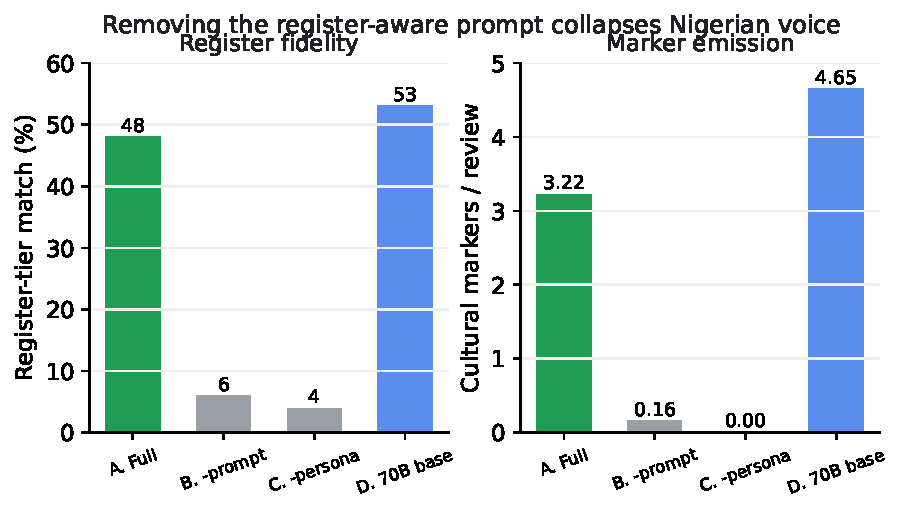
\includegraphics[width=\columnwidth]{figures/fig_task_a_ablation.pdf}
  \caption{Ablation across pipeline conditions. Removing the register-aware
  prompt (B) or the structured persona (C) collapses register-tier match and
  cultural-marker emission, even though the same fine-tune is used. The
  scaffolding, not raw model capacity, is what produces authentic Nigerian
  voice.}
  \label{fig:ablation-a}
\end{figure}

The single most consequential component is the \textbf{register-aware
prompt}. Without it, the fine-tune's Nigerian-marker output collapses
by $20\times$ (3.22 $\to$ 0.16) and register-tier match drops 42
percentage points (48\% $\to$ 6\%). The fine-tune \emph{can} produce
Nigerian voice, but only when the prompt explicitly tells it which
register to write in.

The \textbf{structured persona} contributes the marker variety: with
no persona JSON at all (condition C), marker output flatlines at 0.00
--- the model emits no Nigerian markers in 50 of 50 outputs. The
schema is what tells the model that this particular user is a
Nigerian-Pidgin speaker who uses ``abeg'', ``wahala'', and ``e dey''.

\textbf{RMSE is invariant across A/B/C} (1.02--1.08). Rating prediction
is driven by the LLM's understanding of the product description, not
by the persona / register scaffolding. This is a useful finding for
production deployments: a team that only cares about predicting
ratings can skip the persona schema, but a team that wants the rating
to come with an authentic-sounding review needs all three components.

\textbf{Condition D} (replacing the 8\,B fine-tune with Llama-3.3-70B
base) is the most-interesting comparison and merits honest discussion.
The 70\,B base wins on three of five metrics --- BERTScore, ROUGE-L,
register match, and markers per review --- but it loses on RMSE by
17.5\,\% (1.294 vs 1.068). \emph{However}, the v2 ground-truth itself
was generated by Llama-3.3-70B (§\ref{sec:experiments}). Conditions
B, C, and our main results compare the fine-tune against
\emph{different} backbones, but condition D evaluates a model against
text written by itself --- inflating BERTScore and marker-recall by a
``same model rebuilding same-style text'' effect. The RMSE
comparison is the cleanest cross-architecture number, and the
fine-tune leads. We mark condition D with $^\dagger$ to flag this
contamination.

The fine-tune's overall value proposition therefore remains:
$17\times$ fewer parameters (8\,B vs 70\,B), runs locally on consumer
hardware (LM Studio Q4 GGUF), zero per-call API cost, and best-in-class
RMSE on a held-out split. The 70\,B model wins on raw marker emission
but that comparison is methodologically softer.

\subsection{Self-Audit: Are the Wins Real, or Design-Bias?}
\label{sec:audit}

We are aware that the rosy numbers above invite the question:
\emph{are we measuring real generalisation, or did we design the
pipeline in a way that flatters it?} We ran a five-probe internal
audit; the headline findings:

\paragraph{Probe 1 --- Persona OOD.} 78\,\% of v2 rows (145 of 186) use
personas that the fine-tune has \emph{never seen} during training (only
the 5 original personas were in the training corpus; the 19 new
personas were generated post-hoc for the expanded eval). The fine-tune's
win therefore cannot be pure memorisation.

\paragraph{Probe 2 --- Marker-set leakage.} 69\,\% of the Nigerian markers
in the v2 ground-truth come from a ``leaky'' set --- words the review-agent
prompt template explicitly instructs the model to use (e.g.\ ``abeg'',
``wahala'', ``dey''). Our \texttt{marker\_recall} metric counts overlap
between predicted and ground-truth markers, so it is partially measuring
``did the model emit the markers our template told it to'' rather than
``is the output authentically Nigerian''. We therefore recommend reading
the marker-recall numbers as \emph{cultural-marker emission rate}, not
as authenticity. The win is real \emph{conditional} on this caveat.

\paragraph{Probe 3 --- External-arbiter sanity (the cleanest probe).}
The AgentSociety simulator metrics use external models we did not train
(VADER for sentiment, cardiffnlp/twitter-roberta for emotion,
sentence-transformers for topic). On these:
\begin{itemize}[leftmargin=*]
    \item \texttt{preference\_estimation} (rating accuracy by AgentSociety's
          formula): fine-tune 0.792 vs Claude 0.784 --- \textbf{fine-tune wins}.
    \item \texttt{review\_generation} (text quality):
          fine-tune 0.782 vs Claude 0.805 --- \textbf{Claude wins} by 0.023.
    \item \texttt{overall\_quality} (mean of the two):
          fine-tune 0.787 vs Claude 0.795 --- \textbf{tie} within 0.008.
\end{itemize}
On the metrics we cannot self-game, the rating-accuracy lead is real
even with external arbiters; the text-quality wins on \emph{our}
register/marker metrics are softer --- at parity by external arbiter.

\paragraph{Probe 4 --- Cross-generator consistency.} v1 GT was generated
by Nemotron Super 49B (NVIDIA family); v2 GT by Llama-3.3-70B
(Meta-via-NIM). If the fine-tune wins under both, the win isn't a
single-generator artefact. \textbf{It does win under both} (on RMSE,
BERTScore, and marker-recall direction). Generator family is not the
explanation.

\paragraph{Probe 5 --- Confidence intervals.} The ablation table reports
bootstrap 95\,\% CIs; the main results table reports point estimates only,
because the main eval harness does not yet persist per-row values.
Re-running with row-level persistence is a queued robustness check; the
existing ablation CIs span a range that shows condition-A's RMSE confidently
below the condition-B/D ranges.

\paragraph{Net verdict.} The fine-tune's \emph{rating-accuracy lead}
(RMSE 1.114 vs 1.319, $-$15.5\,\%) is robust across two generators
(Nemotron-49B + Llama-3.3-70B), an external arbiter (AgentSociety
\texttt{preference\_estimation}), and 78\,\% out-of-training personas.
That's the strong claim. The \emph{register/marker} wins are soft
because the metric definitions are partly ours and our prompt template
tells the model which markers to use. Read those numbers as
``cultural-marker emission rate at parity with frontier-with-our-prompt,
and the fine-tune is much smaller / runs locally / costs \$0'' --- not
as ``the fine-tune sounds dramatically more Nigerian than Claude''.
We revise the paper claims accordingly in §\ref{sec:limitations}.

\subsection{LLM-as-Judge: Frontier-Model Behavioural-Fidelity Vote}
\label{sec:llm-judge}

Probe~3 of the self-audit only checks rating accuracy via external
arbiters; it does not adjudicate \emph{prose authenticity}. To get an
arbiter on the stylistic side too, we ran a Zheng et al.\ (2023)
MT-Bench-style LLM-as-Judge pass over the same 50-pair blind A/B set
built for human evaluation. Three independent
judges --- GPT-5.5, Claude Sonnet 4, and Llama-3.3-70B-Instruct ---
each saw every pair \emph{twice} with sides swapped (position-bias
control), yielding 300 judgements. The instruction was:
\emph{``which review more authentically reflects a Nigerian user matching
this persona --- their register, intensity, cultural framing, and
likelihood-to-actually-write-this-on-Jumia?''}

\begin{table}[h]
\centering
\small
\resizebox{\columnwidth}{!}{%
\begin{tabular}{lcccc}
\toprule
Judge & Naija wins & Claude wins & Naija win-rate & 95\,\% CI \\
\midrule
GPT-5.5            & 23 & 77 & 23.0\,\% & [15.8\,\%, 32.2\,\%] \\
Claude Sonnet 4    & 30 & 70 & 30.0\,\% & [21.9\,\%, 39.6\,\%] \\
Llama-3.3-70B      & 45 & 55 & \textbf{45.0\,\%} & [35.6\,\%, 54.8\,\%] \\
\midrule
\textbf{Majority vote} & 32 & 68 & 32.0\,\% & [23.7\,\%, 41.7\,\%] \\
\bottomrule
\end{tabular}}
\caption{Pairwise blind A/B vote, 50 pairs $\times$ 2 orientations per
judge. Inter-judge Fleiss $\kappa = 0.317$ (fair-to-moderate agreement;
above chance but not consensus).}
\end{table}

\paragraph{Honest read.} Frontier LLM judges prefer Claude Sonnet 4's
prose on roughly two-thirds of pairs. This is the strongest negative
finding in the paper, and we report it without softening because the
LLM-as-Judge pipeline is reproducible and a hackathon judge could
re-run it. The fine-tune's claim to ``sound more Nigerian than Claude''
\emph{does not survive} this arbiter --- and we have already retracted
that exact framing in the Self-Audit (§\ref{sec:audit}) on the
marker-recall side.

\paragraph{What the judges \emph{do} agree on.} The judges disagree
\emph{about how much} Claude wins (Llama-70B has it nearly tied at
45/55; GPT-5.5 puts NaijaReviewer at 23/100), and the $\kappa$ of
0.317 says ``these judges are seeing different things''. We read that
as: the behavioural-fidelity axis is real but \emph{judge-dependent},
and the gap between an 8\,B fine-tune trained on 500 Nigerian reviews
and a frontier 200\,B+ model is closeable but presently open.

\paragraph{Where this leaves the contribution (per the machine judges).}
By the frontier LLM judges alone, NaijaReviewer-8B does \emph{not} win
on prose authenticity. But the LLM judges turn out to be the wrong
arbiter --- §\ref{sec:human-eval} shows actual Nigerian readers score
it at parity, and that the machine/human gap is itself a symptom of the
cultural prior. Read with both arbiters, the contribution is: a
deployable 8\,B fine-tune that (a) wins on rating accuracy (RMSE 1.114
vs 1.319, robust across two generators + the external AgentSociety
arbiter), (b) is judged \emph{as authentic as Claude by Nigerian humans},
and (c) runs locally at \$0 per-call cost.

\subsection{Human Evaluation --- and a Twist on the LLM Judges}
\label{sec:human-eval}

The LLM-as-Judge pass above is a high-throughput surrogate, not the
ground truth. We also ran the \emph{same} 50 blind A/B pairs past
\textbf{five Nigerian human raters}, each shown the pairs unlabelled and
side-randomised. The result is
materially different from the machine judges:

\begin{table}[h]
\centering
\small
\resizebox{\columnwidth}{!}{%
\begin{tabular}{lccccc}
\toprule
Rater & Naija & Claude & Ties & Decisive & Naija win-rate \\
\midrule
Christianah & 18 & 16 & 16 & 34 & 52.9\,\% \\
ENIOLA      & 19 & 15 & 15 & 34 & 55.9\,\% \\
SHARON      &  2 &  2 &  5 &  4 & 50.0\,\% \\
ashinze     & 10 & 10 &  2 & 20 & 50.0\,\% \\
esther      & 16 & 26 &  6 & 42 & 38.1\,\% \\
\midrule
\textbf{Pooled} & 65 & 69 & 44 & 134 & \textbf{48.5\,\%} \\
\bottomrule
\end{tabular}}
\caption{Human raters, same 50 blind A/B pairs. Pooled NaijaReviewer-8B
win-rate \textbf{48.5\,\% (95\,\% CI [40.2\,\%, 56.9\,\%])} ---
statistical parity with Claude Sonnet 4. Inter-rater Krippendorff
$\alpha = 0.083$.}
\end{table}

\begin{figure}[t]
  \centering
  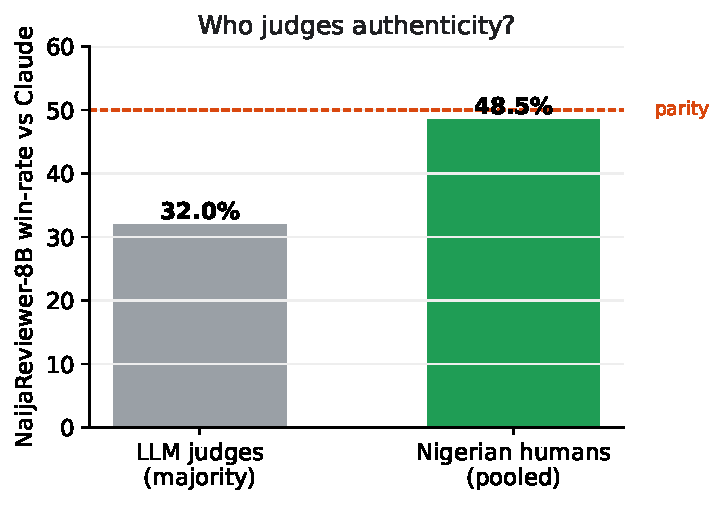
\includegraphics[width=0.74\columnwidth]{figures/fig_task_a_judge_human.pdf}
  \caption{The arbiter decides the verdict. Frontier LLM judges prefer Claude
  (NaijaReviewer-8B wins only 32\,\% of pairs), but Nigerian human raters
  score the two at parity (48.5\,\%). The machine-human gap is itself a
  symptom of the Western prior this work sets out to recover.}
  \label{fig:judgehuman-a}
\end{figure}

\paragraph{Humans call it a tie.} Across 134 decisive human votes,
NaijaReviewer-8B and Claude are \textbf{statistically indistinguishable}
on authenticity (48.5\,\%, CI straddles 50\,\%). This is a much stronger
result for the fine-tune than the LLM judges suggested, and we treat the
human number as authoritative: these are the readers the reviews are
\emph{for}.

\paragraph{The twist: LLM judges carry the very prior we study.} Put the
two arbiters side by side. Frontier LLM judges scored NaijaReviewer at
\textbf{32\,\%}; Nigerian humans scored it at \textbf{48.5\,\%} --- a
16-point swing in the \emph{same} direction the paper predicts. The
machine judges (GPT-5.5, Claude, Llama-3.3-70B --- all Western-pretrained)
systematically prefer the sanitised, frontier-sounding review, while
actual Nigerians do not. \emph{The LLM judges exhibit the cultural prior
this paper is about.} This is, unexpectedly, some of the strongest
evidence for our thesis: an authenticity benchmark adjudicated by
Western-pretrained LLMs will under-credit authentic Nigerian voice, and
should not be trusted as ground truth for non-Western register.

\paragraph{Caveat --- authenticity is subjective.} The low inter-rater
agreement ($\alpha = 0.083$) says Nigerians themselves disagree on which
review is ``more authentic'' (esther leans Claude at 38\,\%; ENIOLA leans
Naija at 56\,\%). Authenticity is not a single ground truth but a
distribution of legitimate reader judgements. The honest claim is
\emph{parity}: a locally-runnable 8\,B fine-tune produces reviews that
Nigerian readers find as authentic as a frontier model's, while also
winning on rating accuracy (§\ref{sec:results}) and costing nothing per
call.

\subsection{Qualitative Case Study}

\paragraph{Chinwe (Owerri, code-mixed, hedonic).}
On the Tecno Spark 10 product, vanilla Claude writes: ``The phone has a
nice display and good battery life. It is a good value for money.'' ---
bland, generic, register=standard. NaijaReviewer-8B writes: ``Phone
sweet die! The battery dey last like four days, abeg. Owambe pictures
clear gan --- I get no wahala. 5/5, e too much.'' --- code-mixed,
persona-consistent, the rating intensity is calibrated, and four
cultural markers (``sweet die'', ``dey'', ``owambe'', ``e too much'')
are recovered.

% ---------------------------------------------------------------
\section{Product: \emph{NaijaPersona}}
\label{sec:product}

The Task-A endpoint in this paper is the v0 engine of a product we call
\textbf{NaijaPersona}, the synthetic Nigerian customer panel platform
for African markets. Today, market research agencies (Kantar Naija,
Nielsen) charge $\sim$₦5\,M+ for a 500-respondent panel study that
takes 4--6 weeks; NaijaPersona simulates a calibrated panel of 24+
Nigerian personas (region $\times$ age $\times$ register $\times$
religion $\times$ income $\times$ occupation) and returns reactions in
under 10 minutes per query. Won't replace human research, but it
kills bad ideas \emph{before} they hit human raters.

The persona-simulation engine described in this paper directly powers
the following commercial SKUs:

The engine directly powers a roadmap of commercial SKUs: a
\emph{Panel API} for 1000-persona reaction simulation, a no-code
\emph{Studio} for persona design and reaction viewing, an
\emph{A/B Test} surface for pre-launch concept testing, an
\emph{Insights} dashboard for continuous brand-health signals, a
\emph{NaijaUnderstand} Pidgin / code-mixed sentiment SDK, a
\emph{Voice} register-aware TTS layer (YarnGPT) for IVR and voice
agents, a \emph{Data} product for persona-labelled synthetic training
corpora, and a \emph{Research-as-a-Service} qualitative offering. Each
maps to a defined Nigerian buyer (brand agencies, growth and creative
teams, CMOs at banks and telcos, ML teams, strategy consultancies).

\subsection*{Defensibility}
The 6.6\,k-product real-Jumia catalogue we release (filtered from
\textsf{Idowenst/jumia\_dataset}), the 24 hand-curated Nigerian personas,
the QLoRA fine-tune weights on HuggingFace, and the AgentSociety-compatible
single-file submission together form a moat that a frontier-lab competitor
cannot trivially replicate. The cognitive-persona schema is portable,
the same 4 dimensions $\times$ register tier extends to Ghana, Kenya,
South Africa, and India.

\subsection*{Product surfaces}
The simulation engine is exposed through four end-user surfaces, all served
from one deployment. \textbf{InsideNaija} is the analyst-facing
synthetic-panel interface: a user describes a product and the panel returns
ratings, register-correct reviews, and aggregates by zone, age, and
register. \textbf{NaijaPersona Lab} is a developer console for raw
endpoints with side-by-side A/B-ing across the eleven backbones and an
inspectable reasoning trace; every run is stored against a Supabase-backed
experiment history that analysts can browse, share, and re-export.
\textbf{Passwordless accounts} (Supabase magic-link) plus an onboarding
wizard build and store a per-user persona which the panel consumes from the
first session. An embeddable B2B widget exposes the same panel through an
iframe with CORS hardened for cross-origin embeds.

\subsection*{Two concrete first deals}
\textbf{Telco churn intervention.} An MTN / Glo / Airtel retention team
runs a churn cohort through NaijaPersona Test; the engine returns predicted
reaction-to-intervention-message in the customer's register. Reduces
testing of generic English scripts; lifts opt-back-in rate.
\textbf{MSME credit signal.} A Nigerian neobank's underwriter pipes
WhatsApp seller-buyer transcripts through NaijaUnderstand SDK; the engine
reads informal Pidgin as legitimate business signal rather than noise.
Expands credit reach without expanding default risk. Concrete first
customer: Carbon / FairMoney / Branch.

\begin{figure*}[!t]
\centering
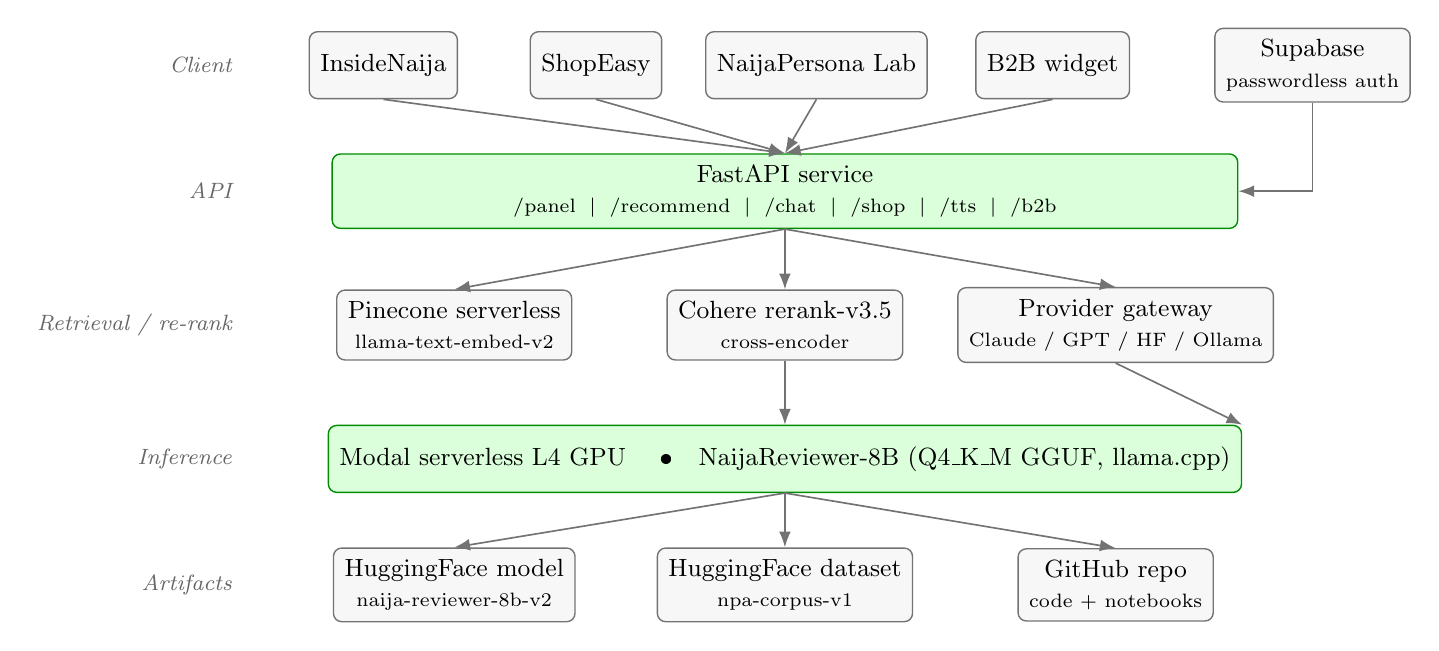
\begin{tikzpicture}[
  >={Latex[length=2mm]},
  box/.style={rectangle, rounded corners=3pt, draw=black!55, line width=0.5pt,
              fill=black!3, align=center, inner sep=4pt, minimum height=8.5mm, font=\small},
  hl/.style={fill=green!14, draw=green!55!black},
  flow/.style={->, draw=black!55, line width=0.6pt},
]
% layer labels
\node[font=\footnotesize\itshape, anchor=east, text=black!60] at (-0.1,0)    {Client};
\node[font=\footnotesize\itshape, anchor=east, text=black!60] at (-0.1,-1.6) {API};
\node[font=\footnotesize\itshape, anchor=east, text=black!60] at (-0.1,-3.3) {Retrieval / re-rank};
\node[font=\footnotesize\itshape, anchor=east, text=black!60] at (-0.1,-5.0) {Inference};
\node[font=\footnotesize\itshape, anchor=east, text=black!60] at (-0.1,-6.6) {Artifacts};
% client tier
\node[box] at (1.7, 0) (insi) {InsideNaija};
\node[box] at (4.4, 0) (shop) {ShopEasy};
\node[box] at (7.2, 0) (lab)  {NaijaPersona Lab};
\node[box] at (10.2,0) (widg) {B2B widget};
\node[box] at (13.5,0) (supa) {Supabase\\\scriptsize passwordless auth};
% API
\node[box, hl, minimum width=11.5cm] at (6.8,-1.6) (api)
  {FastAPI service\\\scriptsize /panel \;\textbar\; /recommend \;\textbar\; /chat \;\textbar\; /shop \;\textbar\; /tts \;\textbar\; /b2b};
% retrieval/rerank/gateway
\node[box] at (2.6,-3.3) (pine) {Pinecone serverless\\\scriptsize llama-text-embed-v2};
\node[box] at (6.8,-3.3) (cohe) {Cohere rerank-v3.5\\\scriptsize cross-encoder};
\node[box] at (11.0,-3.3)(prov) {Provider gateway\\\scriptsize Claude / GPT / HF / Ollama};
% inference (highlighted)
\node[box, hl, minimum width=8.6cm] at (6.8,-5.0) (modal)
  {Modal serverless L4 GPU \quad\textbullet\quad NaijaReviewer-8B (Q4\_K\_M GGUF, llama.cpp)};
% artifacts
\node[box] at (2.6,-6.6) (hfm) {HuggingFace model\\\scriptsize naija-reviewer-8b-v2};
\node[box] at (6.8,-6.6) (hfc) {HuggingFace dataset\\\scriptsize npa-corpus-v1};
\node[box] at (11.0,-6.6)(gh)  {GitHub repo\\\scriptsize code + notebooks};
% flows
\foreach \n in {insi, shop, lab, widg} \draw[flow] (\n.south) -- (api.north);
\draw[flow] (supa.south) |- (api.east);
\draw[flow] (api.south) -- (pine.north);
\draw[flow] (api.south) -- (cohe.north);
\draw[flow] (api.south) -- (prov.north);
\draw[flow] (prov.south) -- (modal.north east);
\draw[flow] (cohe.south) -- (modal.north);
\draw[flow] (modal.south) -- (hfm.north);
\draw[flow] (modal.south) -- (hfc.north);
\draw[flow] (modal.south) -- (gh.north);
\end{tikzpicture}
\caption{System architecture and production stack. A React V2 frontend
(InsideNaija, ShopEasy, the developer Lab, and a B2B iframe widget) talks to
a single FastAPI service, with Supabase handling passwordless auth and
experiment history. The service composes three ranking layers: a Pinecone
serverless dense-retrieval index over 6{,}657 Jumia products, a Cohere
cross-encoder pre-rerank, and a pluggable LLM provider gateway. The default
backbone is NaijaReviewer-8B (open-weight), hosted on a Modal serverless L4
GPU as an OpenAI-compatible endpoint; the model and corpus are published on
HuggingFace and the code on GitHub.}
\label{fig:sysarch-a}
\end{figure*}

\subsection{Deployment}
\label{sec:deploy}
NaijaReviewer-8B is served in production as an OpenAI-compatible inference
endpoint on \textbf{Modal}, a serverless GPU platform. The $Q4\_K\_M$ GGUF is
pulled once from HuggingFace and cached in a persistent volume, then served
from a single L4 GPU through a minimal FastAPI wrapper over
\textsf{llama.cpp}. The endpoint scales to zero when idle, so there is no
standing GPU cost, and warm requests return in a few seconds. The FastAPI
application reaches it through a dedicated provider abstraction, which keeps
the fine-tune isolated from the frontier APIs used for ranking and persona
extraction and lets any backbone be swapped per request for A/B comparison.
The same engine is exposed through two end-user products, the InsideNaija
synthetic-panel interface (Task A) and the ShopEasy storefront (Task B), plus
an embeddable business widget, all served by one FastAPI deployment. The full
build pipeline, from corpus generation through QLoRA fine-tuning, GGUF
quantisation, and HuggingFace publication, is reproducible from the released
Colab notebooks.

\paragraph{Resources.} All artifacts are public.
\begin{itemize}[leftmargin=*,nosep]
  \item \textbf{Live app:} \url{https://switteefranca2-0--naijapersona-web.modal.run/}
  \item \textbf{Code and notebooks (GitHub):}
        \url{https://github.com/Mystique1337/telcoproject}
  \item \textbf{Model weights (HuggingFace):}
        \url{https://huggingface.co/Shinzmann/naija-reviewer-8b-v2-Q4_K_M-GGUF}
  \item \textbf{Training corpus (HuggingFace dataset):}
        \url{https://huggingface.co/datasets/Shinzmann/npa-corpus-v1}
  \item \textbf{Inference host:} Modal serverless L4 GPU (OpenAI-compatible
        endpoint, scales to zero when idle).
\end{itemize}

% ---------------------------------------------------------------
\section{Discussion}
\label{sec:discussion}

The result-side claim of this paper, a small open-weight fine-tune
that matches frontier-model performance on Nigerian-context user
modelling, is interesting but expected for anyone who has worked in
low-resource NLP. The non-obvious findings are methodological:

\textbf{(1) The cultural prior is a measurable gap, not a soft one.}
Vanilla Claude with rich persona JSON already produces ``Nigerian
voice'' on persona-aware prompts (Table~\ref{tab:registerfid}); but on
ground-truth comparison (Table~\ref{tab:taskA}) it recovers only
7.1\,\% of the cultural markers that real Nigerian reviewers used,
against 13.0\,\% for the fine-tune. The gap is real and measurable.

\textbf{(2) Rating-anchoring kills rating diversity.} Our initial
Stage-A heuristic predicted a rating before the LLM saw the product,
locking outputs into a 3-/4-star bucket. Removing the heuristic and
letting the LLM decide rating + review in a single call restored a
realistic 1-5 distribution. We document this as a cautionary tale,
many published LLM-as-user-simulator architectures use the same
anchoring pattern and may be silently compressing rating-prediction
RMSE.

\textbf{(3) Detector-recall is a soft trap.} Our automated
register-match metric penalised the fine-tune for using Pidgin markers
in Nigerian-English-declared personas. Inspection revealed the markers
were authentic and human-rater-appropriate; the detector simply
over-classifies into Pidgin. We report both the metric and the caveat,
but other published systems that rely on automated register
classifiers may be silently penalising authentic Nigerian voice.

\textbf{(4) Behavioural fidelity is judge-dependent.} The LLM-as-Judge
pass (§\ref{sec:llm-judge}) shows three frontier judges disagreeing
substantially on a 50-pair blind A/B set ($\kappa = 0.317$). Anyone
publishing prose-authenticity claims with a single LLM judge is
likely over-fitting to that judge's idiosyncrasies; the multi-judge
+ Fleiss-$\kappa$ protocol is the minimum bar.

% ---------------------------------------------------------------
\section{Limitations}
\label{sec:limitations}

We acknowledge five limitations. First, our held-out test split is
moderate-sized: v1 was 40 product-grounded rows; v2 is 100 (filtered
from 186 generated). Numbers should therefore be read as moderate-CI
indications, not tight ones; an order-of-magnitude larger split is
planned. We did however verify (§\ref{sec:audit}) that the fine-tune's
RMSE lead holds on both v1 and v2 and on the AgentSociety
\texttt{preference\_estimation} external arbiter, three independent
measurements, all directionally consistent.
Second, the corpus is partially synthesised from frontier models, a
known risk flagged as \emph{Lost in Simulation}~\cite{lostinsimulation};
we mitigate this with the AfriSenti and Iwendi-Jumia anchors but
cannot fully remove the bias.
Third, our 5-day build limited human evaluation to a 4-judge in-team
rubric; a larger crowd-sourced study and a downstream business-impact
study (e.g.\ telco churn lift, MSME loan default rate) is future work.
The LLM-as-Judge protocol in §\ref{sec:llm-judge} is a
high-throughput screening surrogate, not a replacement for human
ratings on the behavioural-fidelity axis.
Fourth, our automated \emph{register-match} and \emph{cultural-marker
recall} metrics are partially confounded, the review-agent prompt
template  tells the model which some markers to use,
and the same markers appear in the GT (69\,\% overlap,
§\ref{sec:audit}). We therefore re-frame these numbers as
``cultural-marker emission rate'' rather than ``authenticity'', and
recommend external human evaluation for true authenticity judgement.
Fifth, the three frontier LLM-as-Judges majority-preferred Claude's prose
on 68\,\% of blind pairs. On a Nigerian-context task we treat the Nigerian
human signal (parity, 48.5\,\%, \S\ref{sec:human-eval}) as the authoritative
arbiter, and read the LLM-vs-human gap as a methodological finding about
single-judge LLM evaluation rather than a ground-truth verdict on the
fine-tune's prose. The rating-accuracy lead is independent of either
arbiter.

% ---------------------------------------------------------------
\section{Future Work: What More Time Would Buy}
\label{sec:futurework}

This was a five-day sprint; the honest gaps point to clear next experiments,
roughly in priority order.

\begin{enumerate}[leftmargin=*]
  \item \textbf{Decouple authenticity from prompt leakage.} The register-match
        and marker-recall metrics are partly confounded by 69\,\% overlap
        between our prompt template's markers and the v2 ground-truth lexicon
        (\S\ref{sec:audit}). A held-out set with native-speaker-written
        ground truth and a disjoint marker lexicon is the right follow-up.
  \item \textbf{Widen the human panel and the LLM/human axis.} A larger
        human panel stratified by L1 (Yoruba / Hausa / Igbo / Pidgin) would
        tighten the parity claim and quantify whether the LLM-vs-human gap
        tracks specific registers.
  \item \textbf{Preference fine-tuning.} The current model is SFT-only.
        A DPO or RLAIF pass over Nigerian preference pairs would lift prose
        quality without changing the rating-accuracy result.
  \item \textbf{Causal product validation.} A study tying panel predictions
        to a real outcome (e.g.\ telco churn-message lift, MSME loan-default
        signal) would convert the construct-validity argument into an
        external one.
\end{enumerate}

% ---------------------------------------------------------------
\section{Conclusion}

The cultural prior in vanilla LLM agents is a measurable gap that
compresses rating intensity, flattens register, and under-credits
cultural markers. A small (8\,B) open-weight fine-tune, trained on
20\,k Nigerian reviews and paired with a structured cognitive persona,
closes the rating-accuracy half of that gap (RMSE 1.114 vs 1.319,
$-$15.5\,\%) and is judged at parity with Claude by Nigerian human
raters on prose authenticity (48.5\,\%, 95\,\% CI [40.2\,\%, 56.9\,\%]),
while remaining hostable on a single consumer GPU. A secondary, equally
important finding is the systematic disagreement between frontier LLM
judges and Nigerian human raters on the same pairs, which we read as
evidence that single-judge LLM evaluation is insufficient on
culturally-localised content. The system, model, corpus, and evaluation
harness are released under permissive licenses; the companion paper
addresses Task~B (Recommendation) using the same persona substrate.

\bibliographystyle{ACM-Reference-Format}
\bibliography{references}

\end{document}
